\subsection{Anschlusstechnik}

\subsubsection{Was ist ein balanced Kabel?}
\notebox{Im deutschen heißen balanced Kabel symmetrisch und unbalanced asymetrisch.}
Ein balanced Kabel besteht in unserem Fall meist aus 3 Strängen, 2 für Audioübertragung une einer Erdung (Ground). Die Audioübertragung in den beiden Kabelsträngen wird einmal gespiegelt und daraufhin parallel durch das Kabel geschickt. Wenn eine Störung auftritt wird es in beiden Strängen zeitgleich auftreten und durch die Spiegelung nachträglich wieder zusammengefügt. Da die Störung in die gleiche Richtung auftritt, wird  eine nach der Rückspiegelung ebenfalls gespiegelt. Wenn man nun beide Signale wieder zusammenführt ergibt sich ein Signal wo sich die Störung gegenseitig auslöscht.
\includegraphics[width=1\textwidth]{Bilder/Medientechnik/darstellung Störug.png}\newpage
Bei der Zusammenführung sieht das dann so ungefähr aus, die Spuren werden wieder im Original zusammengelegt (eine zurück gespiegelt) und daraufhin aufaddiert. \\
\includegraphics[width=1\textwidth]{Bilder/Medientechnik/darstellung Störug2.png}

\subsubsection{Beispiele an Anschlusstechnik}
\paragraph{XLR}
~
\begin{figure}[h]
    \centering
    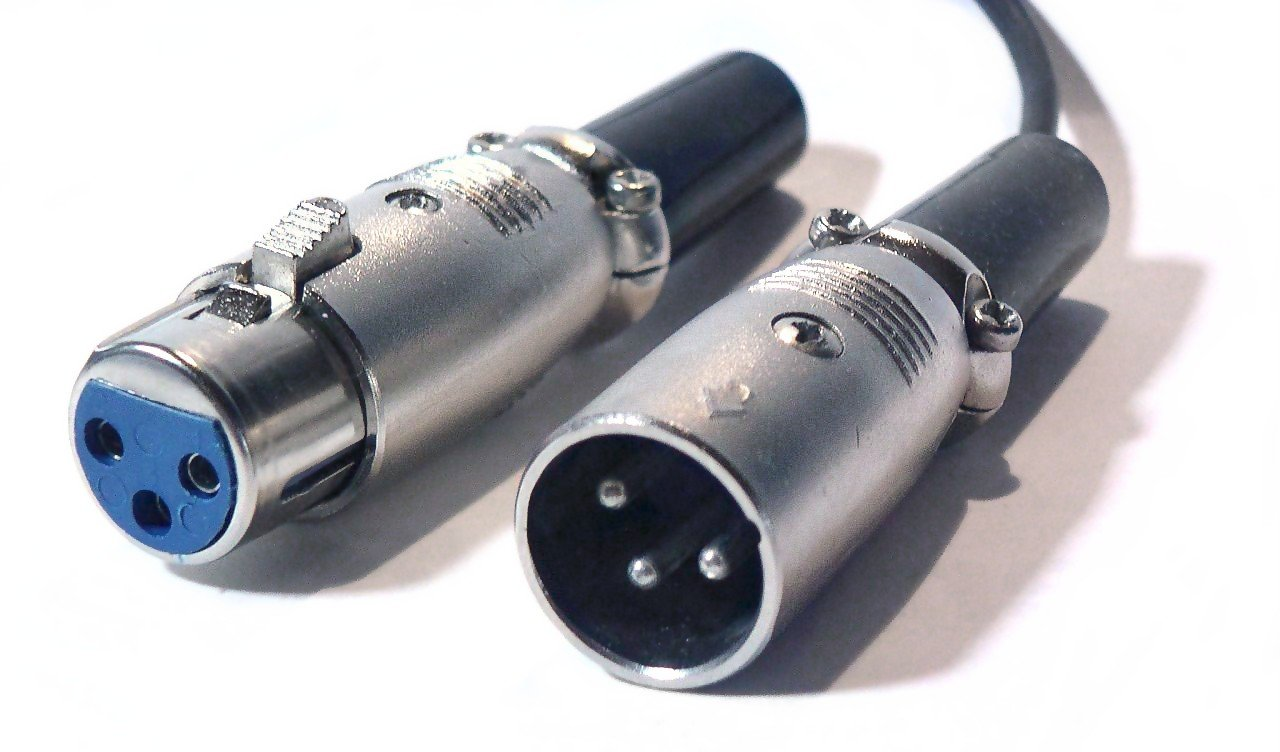
\includegraphics[width=1\textwidth]{Bilder/Medientechnik/Xlr-connectors.jpg}
    \caption{XLR Stecker und Buchse, Bild von Michael Piotrowski\cite{Xlrconne26:online}}
    \label{fig:XLR Stecker \& Buchse}
\end{figure}

links: female, Buchse rechts: male, Stecker\\

XLR steht für \textit{E\textbf{x}ternal \textbf{L}ive \textbf{R}eturn} \cite{AllesXLR:online}, wobei External auch Xcreen/Screen für Masse, Live/Line für Signalübertragungkabel/heiß und Return für Ruckleiterkabel/kalt steht.

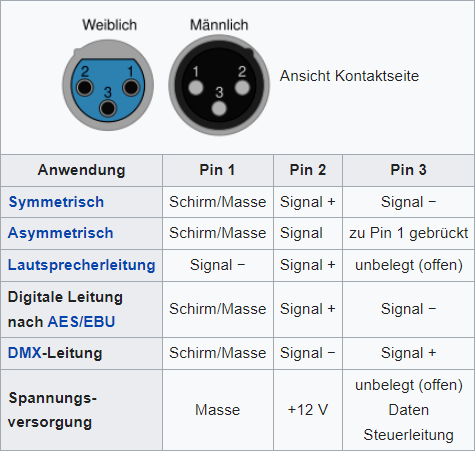
\includegraphics[width=1\textwidth]{Bilder/Medientechnik/XLR-Tabelle.png} \cite{dewiki:241460075}
diese Tabelle zeigt die verschiedenen Konfigurationen eines 3-Poligen-XLR-Kabeln. Diese werden meist im Audiobereich verwendet. Es gibt jedoch auch XLR-Kabel mit bis zu 10-Polen, auch andere Kabel wie DMX (Lichtechnik) nutzen das gleiche Format sind jedoch nicht kompatibel.

\paragraph{Klinkenstecker}
Klinkenstecker gibt es in vielen verschieden Bauarten, jedoch ist ihr Aufbau grundlegend gleich. Sie haben verschieden Größen (Durchmesser): 2,5mm 3,5mm 5,23mm 6,35mm und 7,13mm, die jedoch meist für uns relevanten sind \textbf{6,35mm} für den profesionellen Audiobereich und \textbf{3,5mm} meist für den Heimbereich.\\
Im Aufbau unterscheiden diese sich in der Anzahl an Polen, die Bezeichnung dieser hängt auch von der Anzahl ab. T, R und S sind die kürzel für \textbf{T}ip, \textbf{R}ing und \textbf{S}leeve.\\

\begin{longtable}{|p{0.2\textwidth}|p{0.3\textwidth}|p{0.5\textwidth}|}
\hline
\rowcolor{gray!50} Bezeichnung & Abgeleitet von & Verwendung für \\
\hline
\endfirsthead

\hline
Header 1 & Header 2 & Header 3 \\
\hline
\endhead

\hline
\endfoot

\hline
\endlastfoot

TS & Tip + Sleeve & Monostecker \\
\hline
TRS & Tip + Ring + Sleeve & Stereostecker oder einkanalige sym- metrische Signalübertragung \\
\hline
TRRS & Tip + Ring + Ring + Sleeve & Stecker mit Zusatzkontakt ~~~~(typisch: Mikrofon oder Video) \\
\hline
TRRRS & RTip + Ring + Ring + Ring + Sleeve & Stecker mit Zusatzkontakt ~~~~(typisch: Antischall) \\
\hline

\end{longtable}
\cite{dewiki:245747795}


\begin{figure}[h]
    \centering
    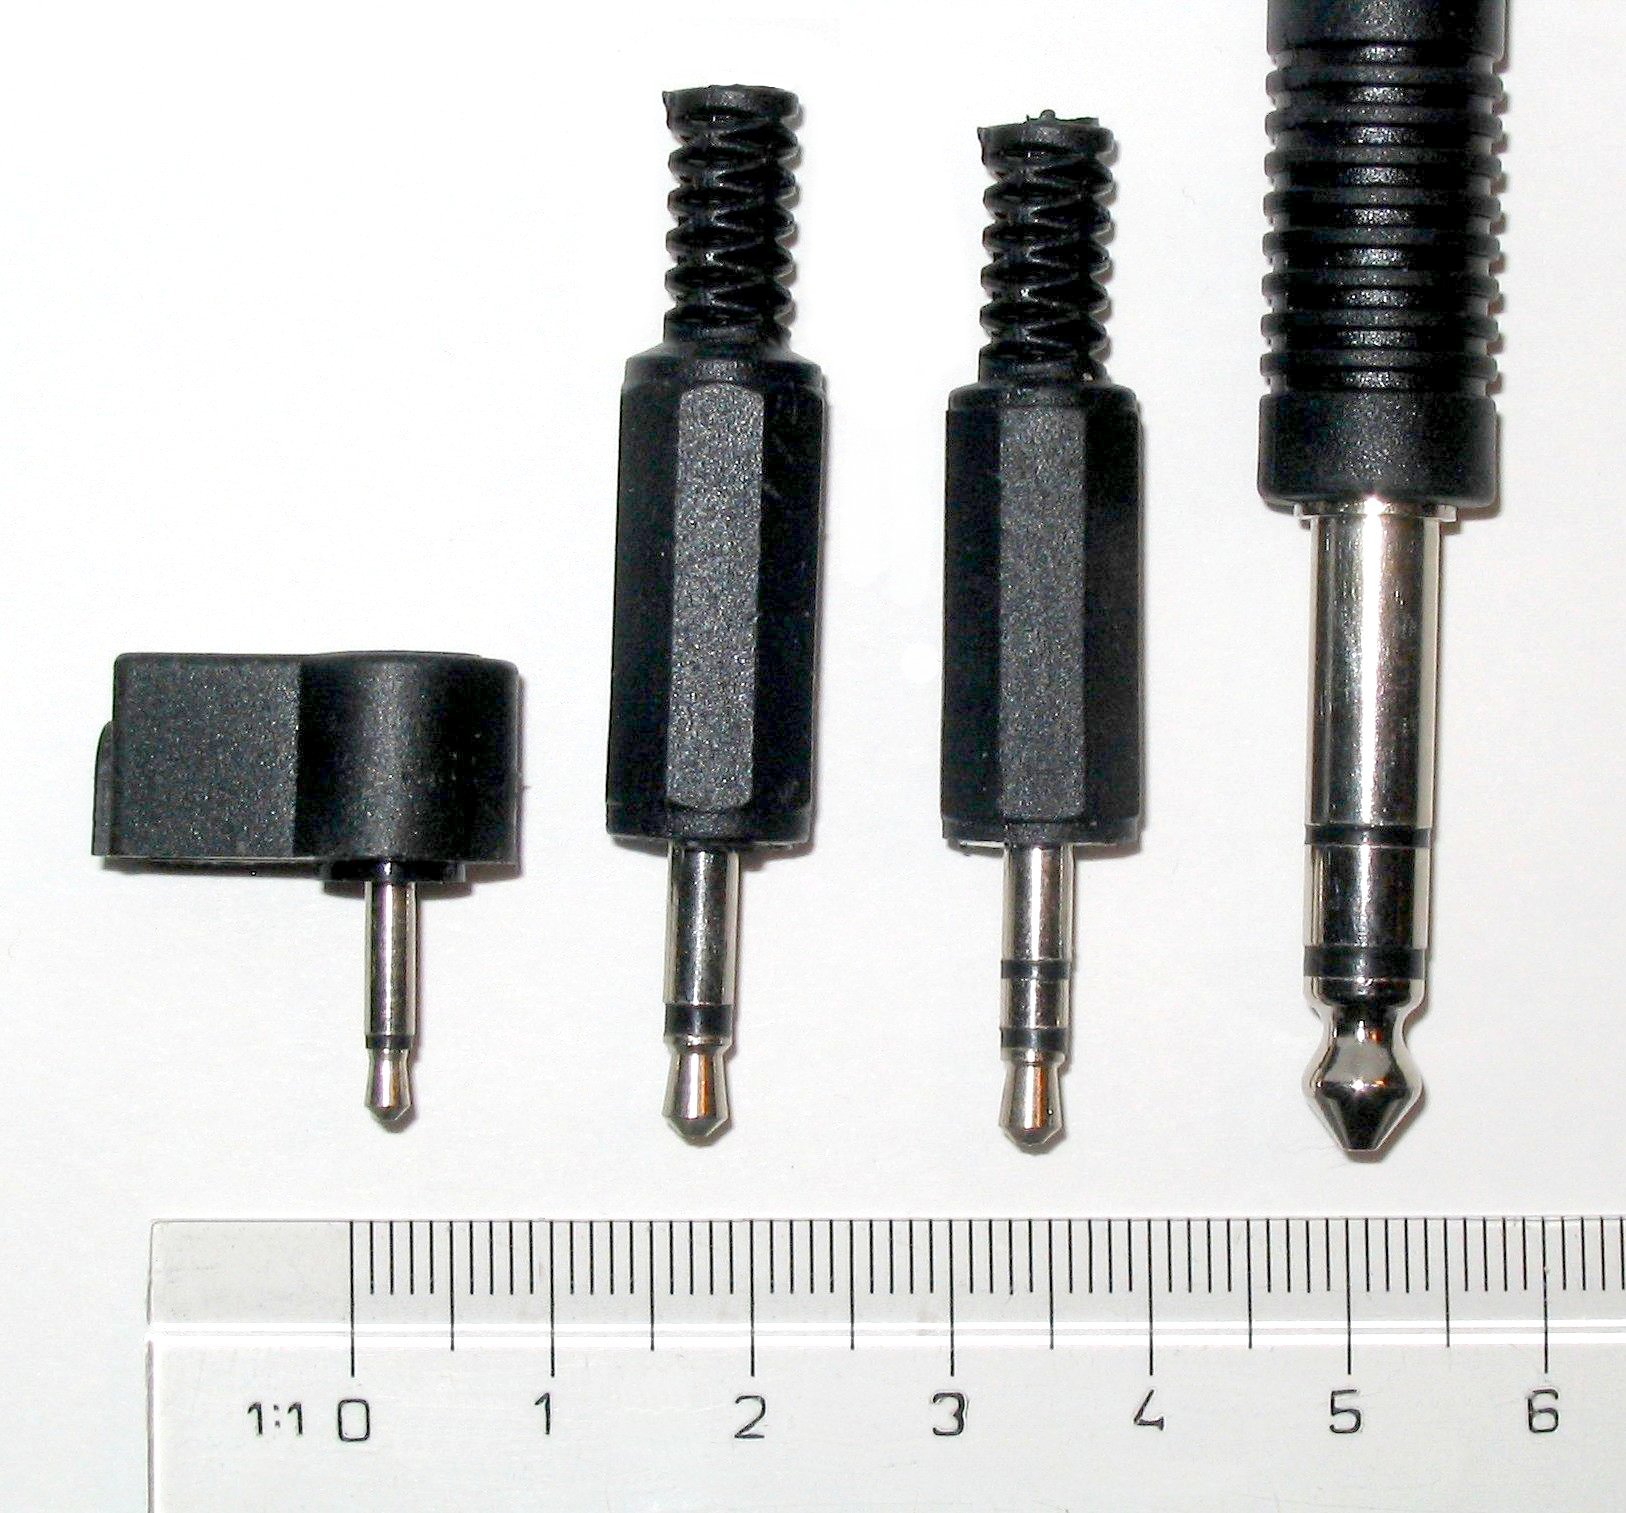
\includegraphics[width=1\textwidth]{Bilder/Medientechnik/Photo-audiojacks.jpg}
    \caption{Beispiele von Klinkensteckern}
    \label{fig:Klinkenstecker}
\end{figure}
\newpage

\paragraph{Chinch}
\includegraphics[]{}



\paragraph{Multicore-Kabel}
\includegraphics[]{}